\chapter{Introducción}
Actualmente, los usuarios que consumimos contenido multimedia contamos con una amplia y actualizada selección a nuestro alcance. Sin embargo, y cada vez más, muchas personas recurren a contenidos, formatos y diseños que hace poco se consideraban anticuados. Ejemplos de este fenómeno, que muestran la preferencia de los usuarios por lo \textit{retro}, incluyen el resurgimiento de los discos de vinilo\footnote{https://www.xataka.com/musica/vinilo-resurge-definitivamente-34-anos-despues-logra-vender-que-formato-cd-ee-uu-espana-tiene-40-cuota} y el deseo de numerosos aficionados a la fotografía de disfrutar de su {\it hobby} a través de medios analógicos\footnote{https://garage.hp.com/us/en/modern-life/analog-film-photography-trend-low-tech-photos.html}. La demanda por parte del público de revisitar y reconsiderar lo ``antiguo'' ha incrementado considerablemente. 

Una de las áreas que más se ha visto beneficiada ha sido la de los videojuegos. Hardware técnicamente desfasado y software con décadas sin soporte oficial han pasado a tener una segunda vida en manos de la comunidad de videojuegos, la cual ha facilitado toda la información y documentación necesaria para que nuevos usuarios puedan participar y jugar. Entre los movimientos que han aparecido se encuentra el {\it homebrew}, software creado por los aficionados para hardware propietario.

Un dato que refuerza lo que comentamos en el párrafo anterior es la respuesta a la demanda por parte de compañías como Nintendo o Sony. Ambas sacaron al mercado revisiones de consolas como las NES, SNES y PlayStation original junto con recopilaciones de juegos tradicionales de los 80 y 90. Cabe mencionar que las dos revisiones de Nintendo tuvieron un gran éxito.

Inevitablemente, la reaparición de este tipo de tecnología puede llegar a generar dudas sobre el porqué de este fenómeno. Una de las razones principales, además de contar con una comunidad dedicada \cite{bib:paper3}, es la relativa facilidad para iniciarse: Mientras que para el hardware más actual es necesario invertir tiempo y dinero en adquirir (y aprender a utilizar) SDK's oficiales y frameworks, el hardware antiguo ofrece gran cantidad de documentación pública y, en la mayoría de casos, numerosos emuladores que además de facilitar el desarrollo de juegos, ofrecen al jugador diversas formas de jugar. Esto último es otra razón por la que es llamativo desarrollar para este tipo de hardware. Por ejemplo, un juego desarrollado para la NES estará disponible para una gran variedad de sistemas (cualquiera que cuente con un emulador de NES en este caso).

Sin embargo, además del punto de vista práctico, desarrollar para máquinas {\it retro} también puede resultar atractivo con fines educativos. Un ejemplo de ello puede ser \cite{bib:paper_1}, donde los autores exploran el uso de micro-proyectos de CHIP-8, una plataforma de videojuegos de los 80, para aplicarlos en distintas asignaturas del grado de Ingeniería Informática. Más ejemplos de aplicación didáctica pueden encontrarse en \cite{bib:paper_2}, donde el autor habla sobre el uso de la Game Boy Advance, la popular consola portátil de principios del 2000, para enseñar Arquitectura de Computadores y \cite{bib:paper3}, donde los autores diseñan un curso alrededor de la Game Boy Advance y su sucesora, la Nintendo DS, para enseñar programación a sus alumnos. De forma adicional, en \cite{bib:paper_5} se comenta, entre otras cosas, el rol que tiene el desarrollo \textit{amateur} de videojuegos al adquirir nuevas habilidades y conocimientos. Programar para este tipo de dispositivos requiere un cierto conocimiento del hardware que en otras áreas no es necesario. Para sacarle el máximo partido al hardware (especialmente cuando se trata de hardware con especificaciones limitadas) se intenta evitar la programación a altos niveles de abstracción.

Es lo descrito en el párrafo anterior lo que nos lleva al dispositivo que utilizaremos durante este trabajo, la {\bf Game Boy Advance}.

\section{Game Boy Advance}

Con el increíble éxito que tuvo su predecesora, la Game Boy Color, Nintendo decidió sacar una nueva versión de la consola portátil en 2001, mejorando las especificaciones técnicas con las que contaba el modelo anterior y empleando una arquitectura completamente nueva. Hasta el 2010, año en el que Nintendo descatalogó el dispositivo, se lanzaron una gran cantidad de juegos, aproximadamente 1500\footnote{https://nintendo.fandom.com/wiki/List\_of\_Game\_Boy\_Advance\_games}. De forma adicional, se introdujeron dos modelos actualizados del dispositivo original, la Game Boy Advance SP y la Game Boy Advance Micro. Estas conservaban las especificaciones base de la consola pero mejoraban aspectos como la pantalla LCD. Las tres versiones se pueden ver en la Figura \ref{fig:modelos}. Combinando todos los modelos, se vendieron en torno a 80 millones de unidades\footnote{https://www.nintendo.co.jp/ir/pdf/2007/070426e.pdf\#page=21}, convirtiéndose así en una de las consolas más exitosas comercialmente.
\begin{figure}[b]
	\centering
	\begin{subfigure}[h]{0.3\textwidth}
		\centering
		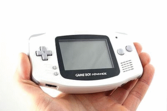
\includegraphics[width=\textwidth]{capitulos/capitulo1/modelo_a.png}
		\label{fig:modelo_a}
		\caption{Game Boy Advance}
	\end{subfigure}
	\hfill
	\begin{subfigure}[h]{0.3\textwidth}
		\centering
		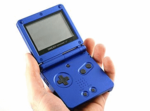
\includegraphics[width=\textwidth]{capitulos/capitulo1/modelo_b.png}
		\label{fig:modelo_b}
		\caption{Game Boy Advance SP}
	\end{subfigure}
	\hfill
	\begin{subfigure}[h]{0.3\textwidth}
		\centering
		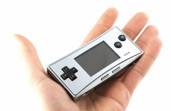
\includegraphics[width=\textwidth]{capitulos/capitulo1/modelo_c.png}
		\label{fig:modelo_c}
		\caption{Game Boy Advance Micro}
	\end{subfigure}
	\caption{Game Boy Advance, Game Boy Advance SP y Game Boy Advance Micro.}
	\label{fig:modelos}
\end{figure}


Entre los factores que contribuyeron a su éxito se incluyen la retrocompatibilidad con la generación de consolas previa de Nintendo, su precio asequible, la calidad de los juegos que desarrollaban las {\it third-party}\footnote{Se conoce como third-party a los juegos desarrollados por una entidad ajena a la compañía propietaria de la plataforma en la que se publican.} o la propia Nintendo y la relativa novedad que todavía tenía el mercado de consolas portátiles. Gracias a todos estos factores, la compañía japonesa prácticamente disfrutó de un monopolio en el mundo de las consolas portátiles\footnote{https://www.theverge.com/2019/4/19/18507409/nintendo-game-boy-competitors-nokia-sony-bandai} (esto se aplica tanto para la Game Boy original como para la Advance). \\ \\

\section{Explicación y objetivos del proyecto}\label{sec:objs}

En este Trabajo Fin de Grado se programará un {\bf juego para la consola Game Boy Advance}, que funcionará en el hardware original\footnote{Se probará con una Nintendo DS Lite, consola retrocompatible con la Game Boy Advance.} y en emuladores. Es importante destacar este aspecto porque el hecho de que un juego funcione en un emulador no garantiza que funcione también en el hardware original. Comentaremos algunos ejemplos de situaciones de este tipo a lo largo del trabajo.

Para poder realizar el proyecto correctamente se precisarán {\bf conocimientos del lenguaje de programación C aplicados a máquinas de propósito específico}. Estos deberán complementarse con un {\bf conocimiento de la arquitectura y funciones propias de la Game Boy Advance}. De forma adicional, dado que el trabajo se especializa en un área como es la de los videojuegos, será necesario {\bf familiarizarse con las técnicas profesionales de desarrollo de videojuegos}. Se espera poder conseguir un producto acorde con la calidad que ha ofrecido durante años la comunidad {\it homebrew}. Algo a destacar en este aspecto es la integración de archivos multimedia para su uso en el producto final. Entre los contenidos que se utilizarán se incluyen tanto {\it sprites}\footnote{Imagen asignada a un objeto/personaje de un videojuego.} como pistas de audio. Finalmente, el trabajo también requerirá del {\bf uso de métricas de rendimiento} durante el desarrollo para poder evaluar el software escrito y tomar decisiones en base a los resultados obtenidos.

En la siguiente lista se muestra  un resumen de los objetivos parciales anteriormente planteados, y derivados del objetivo principal de crear un juego para la Game Boy Advance (abreviada normalmente como GBA):

\begin{itemize}
	\item Aprendizaje de la arquitectura de la Game Boy Advance.
	\item Adquisición de conocimientos de desarrollo para máquinas de propósito específico.
	\item Ampliación práctica del conocimiento sobre programación en lenguaje C.
	\item Familiarización con las técnicas profesionales de desarrollo de videojuegos.
	\item Aplicación de técnicas de programación eficiente apoyadas en medidas de rendimiento (benchmarking) para comparar estrategias y soluciones a un mismo problema.
\end{itemize}

\section{Justificación e Intereses}

La idea de desarrollar un juego para una consola antigua, descatalogada desde hace más de una década, puede parecer un tanto peculiar como proyecto. Sin embargo, se puede justificar en base a diversos motivos. Uno de ellos es la arquitectura ARM\cite{bib:arm_book} de la máquina escogida, cuya relevancia no deja de aumentar actualmente. Otra razón es el atractivo docente de la propia consola, que permite estudiar, en un mismo dispositivo, muchos conceptos presentes en los planes de estudio del Grado en Ingeniería Informática \cite{bib:paper_2}. Igualmente, el trabajo no deja de precisar del esfuerzo y dedicación que cualquier proyecto de software requiere. Las labores de planteamiento, realización y gestión siguen estando presentes, e incluso se pueden llegar a dificultar dadas las peculiaridades que presenta un dispositivo de este tipo. Para poder realizar un proyecto de este estilo, el programador tendrá que involucrarse tanto en los aspectos más técnicos que trae consigo la programación de un dispositivo empotrado, como el diseño de funcionalidades con las que el usuario interactuará y que son ajenas a la programación (por lo menos de forma directa), como son el diseño de menús, personajes, niveles y controles del juego.

Además, el interés no solo procede de las dificultades que presentará la realización del trabajo, sino del dispositivo en sí. A título personal, el autor de este trabajo ha estado desde su infancia en contacto con consolas del fabricante nipón. Vivió incluso el final de la época de esplendor de la GBA. Por este motivo, poder desarrollar ahora software para esta plataforma supone un importante factor motivador. De forma complementaria, el desarrollo de software para sistemas empotrados siempre ha sido otro tema de interés para el autor dada su experiencia previa con microcontroladores ESPRESSIF\cite{doi:10.1177/0020294019857748} y Arduino. De hecho, desarrolló para el primero un pequeño juego, por lo que la transición a la Game Boy Advance se podría considerar el siguiente paso a seguir para continuar afianzando los conocimientos adquiridos.

Otro aspecto que motiva la realización de este trabajo, y que puede parecer contradictorio dada la naturaleza del dispositivo, es la disponibilidad del producto final para una infinidad de plataformas. Tal y como ya se mencionó, el software desarrollado podrá ejecutarse realmente en casi cualquier dispositivo actual gracias a la popularidad de la emulación.

En base a lo expuesto, podemos concluir que la realización del proyecto supone una motivación personal para el autor. Es además una propuesta bastante original en comparación a otros trabajos de este tipo aunque tenga las mismas exigencias a efectos prácticos. Igualmente, el resultado se podrá usar sin problemas en entornos actuales a pesar de estar destinado a una máquina descatalogada. Por consiguiente, se considera una forma perfecta de certificar los conocimientos y competencias adquiridas durante el Grado en Ingeniería Informática.

\section{Planificación del proyecto}
En este apartado se mostrarán las tareas a realizar y su planificación para completar los objetivos propuestos en la sección \ref{sec:objs}. La realización de las tareas se hará de modo que se siga una \textbf{estrategia de desarrollo} similar al \textbf{Ágil} (metodología popular en la industria de videojuegos \cite{bib:paper6,bib:agile_course}), en la que existirán varias iteraciones y prototipos del juego. Cada nueva iteración tendrá como base el \textit{feedback} y conocimientos adquiridos en la iteración anterior con el objetivo de conseguir un producto final pulido y acorde con los objetivos establecidos. Las diferentes fases de cada iteración se pueden observar en la Figura \ref{fig:agile}.

\begin{figure}[h]
	\centering
	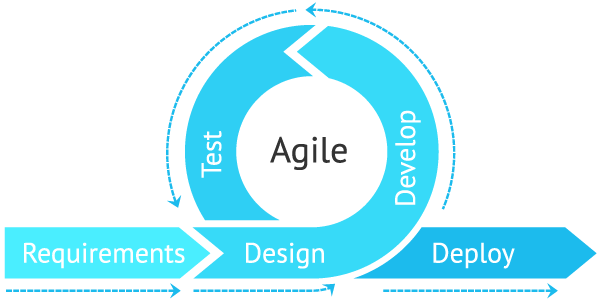
\includegraphics[width=.4\textwidth]{capitulos/capitulo1/agile.png}
	\caption[Metodología ágil]{Metodología ágil. Imagen de \url{devcom.com}.}
	\label{fig:agile}
\end{figure}

En su forma más simplificada, cada iteración repetirá el proceso del modelo de desarrollo en cascada, con la diferencia de que la metodología ágil no requiere acabar completamente cada fase. Por lo tanto, una vez planteado el proyecto y sus especificaciones (\textit{Requirements} en la Figura \ref{fig:agile}), las fases restantes se compondrán de las siguientes etapas:

\begin{enumerate}
	\item Diseño: Teniendo en cuenta los objetivos del proyecto, se diseñarán nuevas especificaciones y funcionalidades a implementar en la iteración actual.
	\item Desarrollo: Se implementará lo especificado en la fase anterior.
	\item Pruebas: Se evaluará lo desarrollado en el punto 2, comprobando que funciona acorde a lo esperado, tanto a nivel de programación, como a nivel conceptual, siendo habitual la prueba por parte del usuario final.
	\item Revisión: A pesar de que normalmente se incluye en la fase de Pruebas, esta fase merece una mención aparte. Teniendo en cuenta, los constantes cambios que se realizan en este tipo de proyectos, es necesario revisar lo desarrollado y decidir si el proyecto sigue acorde con la idea original. Los ajustes a realizar se identificarán en esta fase y se tendrán en cuenta para la próxima iteración.
\end{enumerate}

Con una versión del producto acabada, los desarrolladores publicarán la iteración con la posibilidad de empezar a revisitar las fases descritas anteriormente para lanzar una versión mejorada o con más funcionalidades \cite{bib:agile_course}.

Dado que el proyecto se comenzó con un escaso conocimiento sobre las funcionalidades y arquitectura de la Game Boy Advance, se aprovecharon las iteraciones para conocer las diferentes opciones y características del dispositivo. Por ejemplo, en la primera iteración se analizaron las posibilidades a nivel gráfico que ofrece el dispositivo, mientras que durante la segunda iteración se exploraron las posibilidades que ofrece el procesador, a nivel de audio. En total, se utilizaron un total de 4 iteraciones, también denominadas \textit{sprints}, para realizar el proyecto.

Al combinar los \textit{sprints} junto con las demás tareas ``no iterables'' se obtiene un proyecto el cual ha requerido \textbf{300 horas en total}. Las tareas en cuestión se distribuyen de la siguiente manera:

\begin{enumerate}
	\item \textbf{Estudio de la arquitectura de la Game Boy Advance (40 horas)}: Estudio de la arquitectura con ayuda de la documentación recogida en la bibliografía.
	\item \textbf{Asimilación de técnicas de programación específicas (18 horas)}: Estudio de proyectos de código abierto para Game Boy Advance con los que aprender estrategias de desarrollo de calidad contrastada para esta plataforma.
	\item \textbf{\textit{Sprint} (49.25 horas)}: Desarrollo del proyecto. A continuación, se desglosan y describen las tareas de cada uno de los 4 \textit{sprints} que se realizan, para un total de 197 horas.
		\begin{itemize}
			\item \textbf{Reuniones con los tutores (20 horas)}: Reuniones con el profesorado para definir los requisitos del proyecto, seguir su desarrollo y resolver posibles dudas.
			\item \textbf{Diseño de los niveles del juego (17 horas)}: Estudio de niveles existentes en diferentes juegos para inspiración propia.
			\item \textbf{Diseño y creación de recursos (5 horas)}: Elaboración, mediante herramientas como Adobe Photoshop o GIMP, de elementos del juego como sprites e iconos. Dada la poca familiaridad con el software de dibujo y la falta de experiencia en este campo, se propuso optar por diseños \textit{Open Source} para realizar el juego. A pesar de trabajar con recursos ya existentes, se siguen necesitando 5 horas, dado que será necesario convertirlos a formatos que la consola pueda ``entender''.
			\item \textbf{Implementación (105 horas)}: Programación del juego deseado acorde a las especificaciones propuestas en las tareas de ``Diseño''. Esta tarea es la más exigente, por lo que se le asignaron un mayor número de horas que a las restantes. 
			\item \textbf{Evaluación del producto (50 horas)}: Análisis del resultado obtenido en la tarea de ``Implementación'' para la identificación y solución de errores y aplicación de mejoras.
		\end{itemize}
	\item \textbf{Elaboración de memoria (45 horas)}: Redacción de un informe que describa todo el trabajo desarrollado en las distintas facetas.
\end{enumerate}

La temporización de las tareas mostradas se puede observar en la Tabla~\ref{tab:iteraciones}. Por su parte, el diagrama de Gantt, que refleja visualmente los datos mostrados en la Tabla~\ref{tab:iteraciones}, quedaría como se muestra en la Figura~\ref{fig:gantt}. La Tabla se ha calculado estimando unas 2 horas por día dedicadas al proyecto. 

\begin{table}[h]
	\centering
	\begin{tabular}{| l | l | l | l |}
		\hline
		\textbf{Tarea} & \textbf{Duración} & \textbf{Inicio} & \textbf{Fin} \\ \hline
		Estudio arquitectura GBA & 40 horas & Lunes 08/02/21 & Sábado 27/02/21 \\ \hline
		Estudio técnicas de programación & 18 horas & Domingo 28/02/21  & Lunes 08/03/21\\ \hline
		Sprint 1 & 49.25 horas & Martes 09/03/21 & Sábado 03/04/21 \\ \hline
		Sprint 2 & 49.25 horas & Sábado 03/04/21 & Miércoles 28/04/21 \\ \hline
		Sprint 3 & 49.25 horas & Miércoles 28/04/21 & Domingo 23/05/21 \\ \hline
		Sprint 4 & 49.25 horas & Domingo 23/05/21 & Jueves 17/06/21 \\ \hline
		Elaboración del informe & 45 horas & Jueves 17/06/21 & Viernes 09/07/21 \\ \hline
		Entrega & - & \multicolumn{2}{c|}{Viernes 09/07/21} \\ \hline
	\end{tabular}
	\caption{Temporización por iteración.}
	\label{tab:iteraciones}
\end{table}

\begin{figure}[t]
	\centering
	\rotatebox[origin=c]{270}{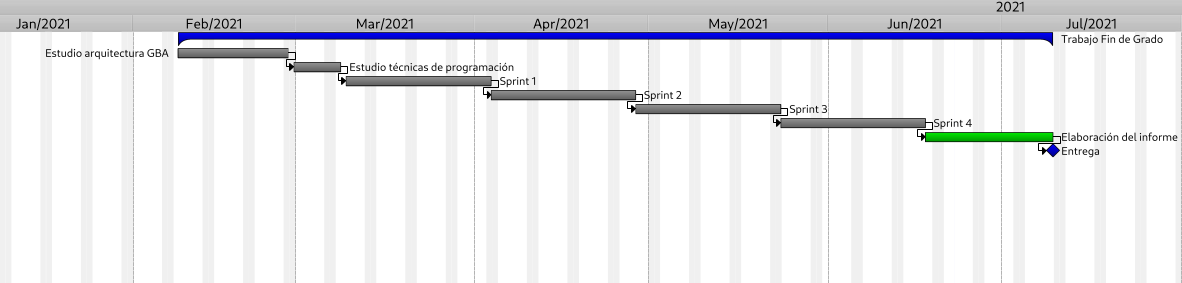
\includegraphics[width=20cm]{capitulos/capitulo1/gantt_3.png}}
	%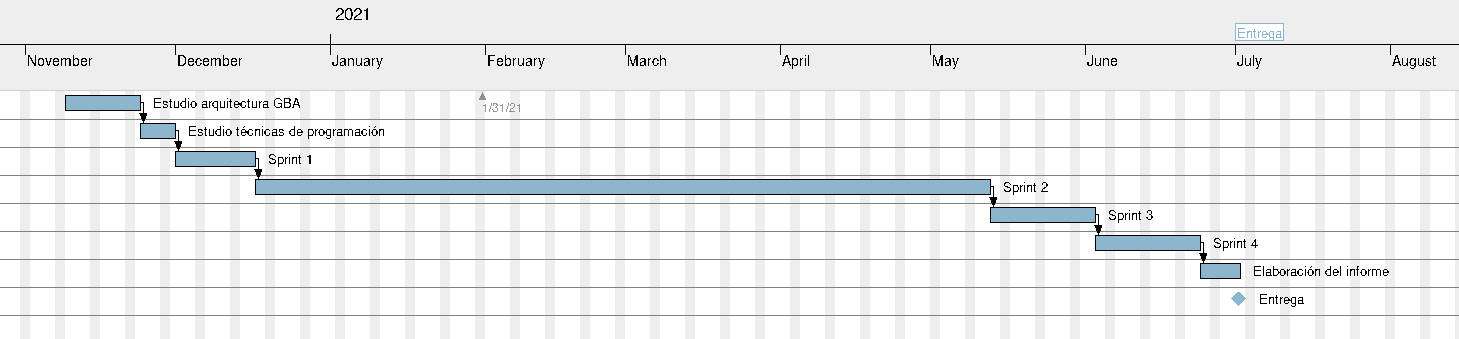
\includegraphics[height=1.2\textwidth]{capitulos/capitulo1/gantt_2.png}
	\caption{Diagrama de Gantt.}
	\label{fig:gantt}
\end{figure}
\FloatBarrier{}

\section{Recursos utilizados}
En esta sección se describirán las herramientas utilizadas para poder realizar satisfactoriamente el proyecto. Se ha considerado oportuno clasificarlas en los subapartados de Lenguajes de programación, Control de versiones, Editores, Herramientas gráficas y de audio, Herramientas de planificación, Emuladores y Hardware.

\subsection{Lenguajes de programación}
Como se mencionó en el punto \ref{sec:objs}, para llevar a cabo el proyecto se va a \textbf{programar en C}. Aunque actualmente existen varias formas de desarrollar un juego para la Game Boy Advance (a partir de C++ y Rust por ejemplo), se seguirá apostando por C, dada la documentación y su uso extendido en la comunidad \textit{homebrew}. El estándar utilizado para el proyecto será el ``GNU17'', el que usa GCC por defecto\footnote{https://gcc.gnu.org/onlinedocs/gcc-11.1.0/gcc/Standards.html}, que es también el compilador empleado en este proyecto. Además, para simplificar el proceso de compilación, se hará uso de la utilidad make.

\subsection{Control de versiones}
Para gestionar el código se hará uso del popular software de control de versiones \textbf{Git}. Además, para alojar el proyecto se utilizará un servidor privado (de modalidad gratuita) de \textbf{\href{https://github.com/}{GitHub}}.

\subsection{Editores}
Dada la necesidad de programar y escribir el informe final en diferentes máquinas, se optará por utilizar editores multiplataforma. Para programar se hará uso de \textbf{Vim} y \textbf{Visual Studio Code}. El primero es adecuado para editar rápidamente archivos y automatizar ciertas tareas, mientras que el segundo es muy eficaz para trabajar simultáneamente con diversos archivos.

En cuanto a la escritura del informe, se hará uso de \textbf{\TeX maker}, que proporciona una interfaz simple y cómoda para personas que no cuenten con mucha experiencia escribiendo en \LaTeX.

\subsection{Herramientas gráficas y de audio}\label{sec:herr_graficas}
Teniendo en cuenta la naturaleza del dispositivo para el que se programará, será necesario convertir los diferentes recursos gráficos a un formato especial. \textbf{Grit} y \textbf{SuperFamiconv}, herramientas creadas específicamente para la conversión de imágenes a un formato reconocible por la Game Boy Advance, se utilizarán para adaptar recursos conocidos como \textit{sprite sheets} y \textit{tile sets} (los cuales se explicarán y se verán con más detenimiento en el punto \ref{sec:ppu}).

Independientemente de si los recursos gráficos son de terceros o propios, la mayoría de las veces será necesario retocar las imágenes antes de convertirlas. Para ello será necesario \textbf{Pixelorama}, editor específicamente diseñado para trabajar con \textit{sprites}.

Para generar los fondos que utilizará el juego, se hará uso de \textbf{Tiled}, uno de los editores de niveles \textit{open source} más populares. Su uso se mostrará en el punto \ref{sec:ppu}.

Por último, para convertir música utilizada para el juego en un formato reconocible para el dispositivo se utilizará \textbf{Audacity}.

\subsection{Herramientas de planificación}
Para planificar cada una de las tareas del proyecto así como calcular su distribución se utilizará \textbf{Plan}, de la suite de aplicaciones Calibra. Por otro lado, \textbf{Trello} se utilizará para clasificar las tareas del proyecto en cada uno de los \textit{sprints} a realizar.

\subsection{Emuladores}
Tras explicar las herramientas necesarias para poder desarrollar el proyecto, pasamos a aquellas que nos permitirán probarlo y ejecutarlo. Las escogidas para este proyecto son los emuladores mGBA y No\$GBA. Del primero se destaca su activo desarrollo y el ser multiplataforma, mientras que del segundo se pueden resaltar las opciones de depuración que ofrece al usuario.

%\begin{figure}[h]
%    \centering
%    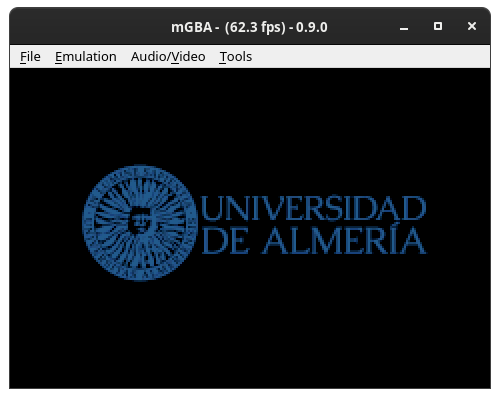
\includegraphics[width=.5\textwidth]{capitulos/capitulo1/mgba.png}
%    \caption{El emulador mGBA.}
%    \label{fig:mgba}
%\end{figure}
%\FloatBarrier

\subsection{Hardware}
Finalmente, pasamos a los recursos que ejecutarán las versiones finales de nuestro proyecto (también las versiones de desarrollo, pero con menor frecuencia). En este caso, al no disponer de una consola Game Boy Advance original, se hará uso de una consola retrocompatible, la \textbf{Nintendo DS Lite} (véase la Figura \ref{fig:nintendo_ds}).

Lamentablemente, la consola no admite cargar directamente software \textit{homebrew}. Por este motivo, se utilizará un cartucho \textbf{Supercard} (véase la Figura \ref{fig:supercard}), que permitirá, mediante una tarjeta microSD, ejecutar el software generado.

\begin{figure}[h]
	\centering
	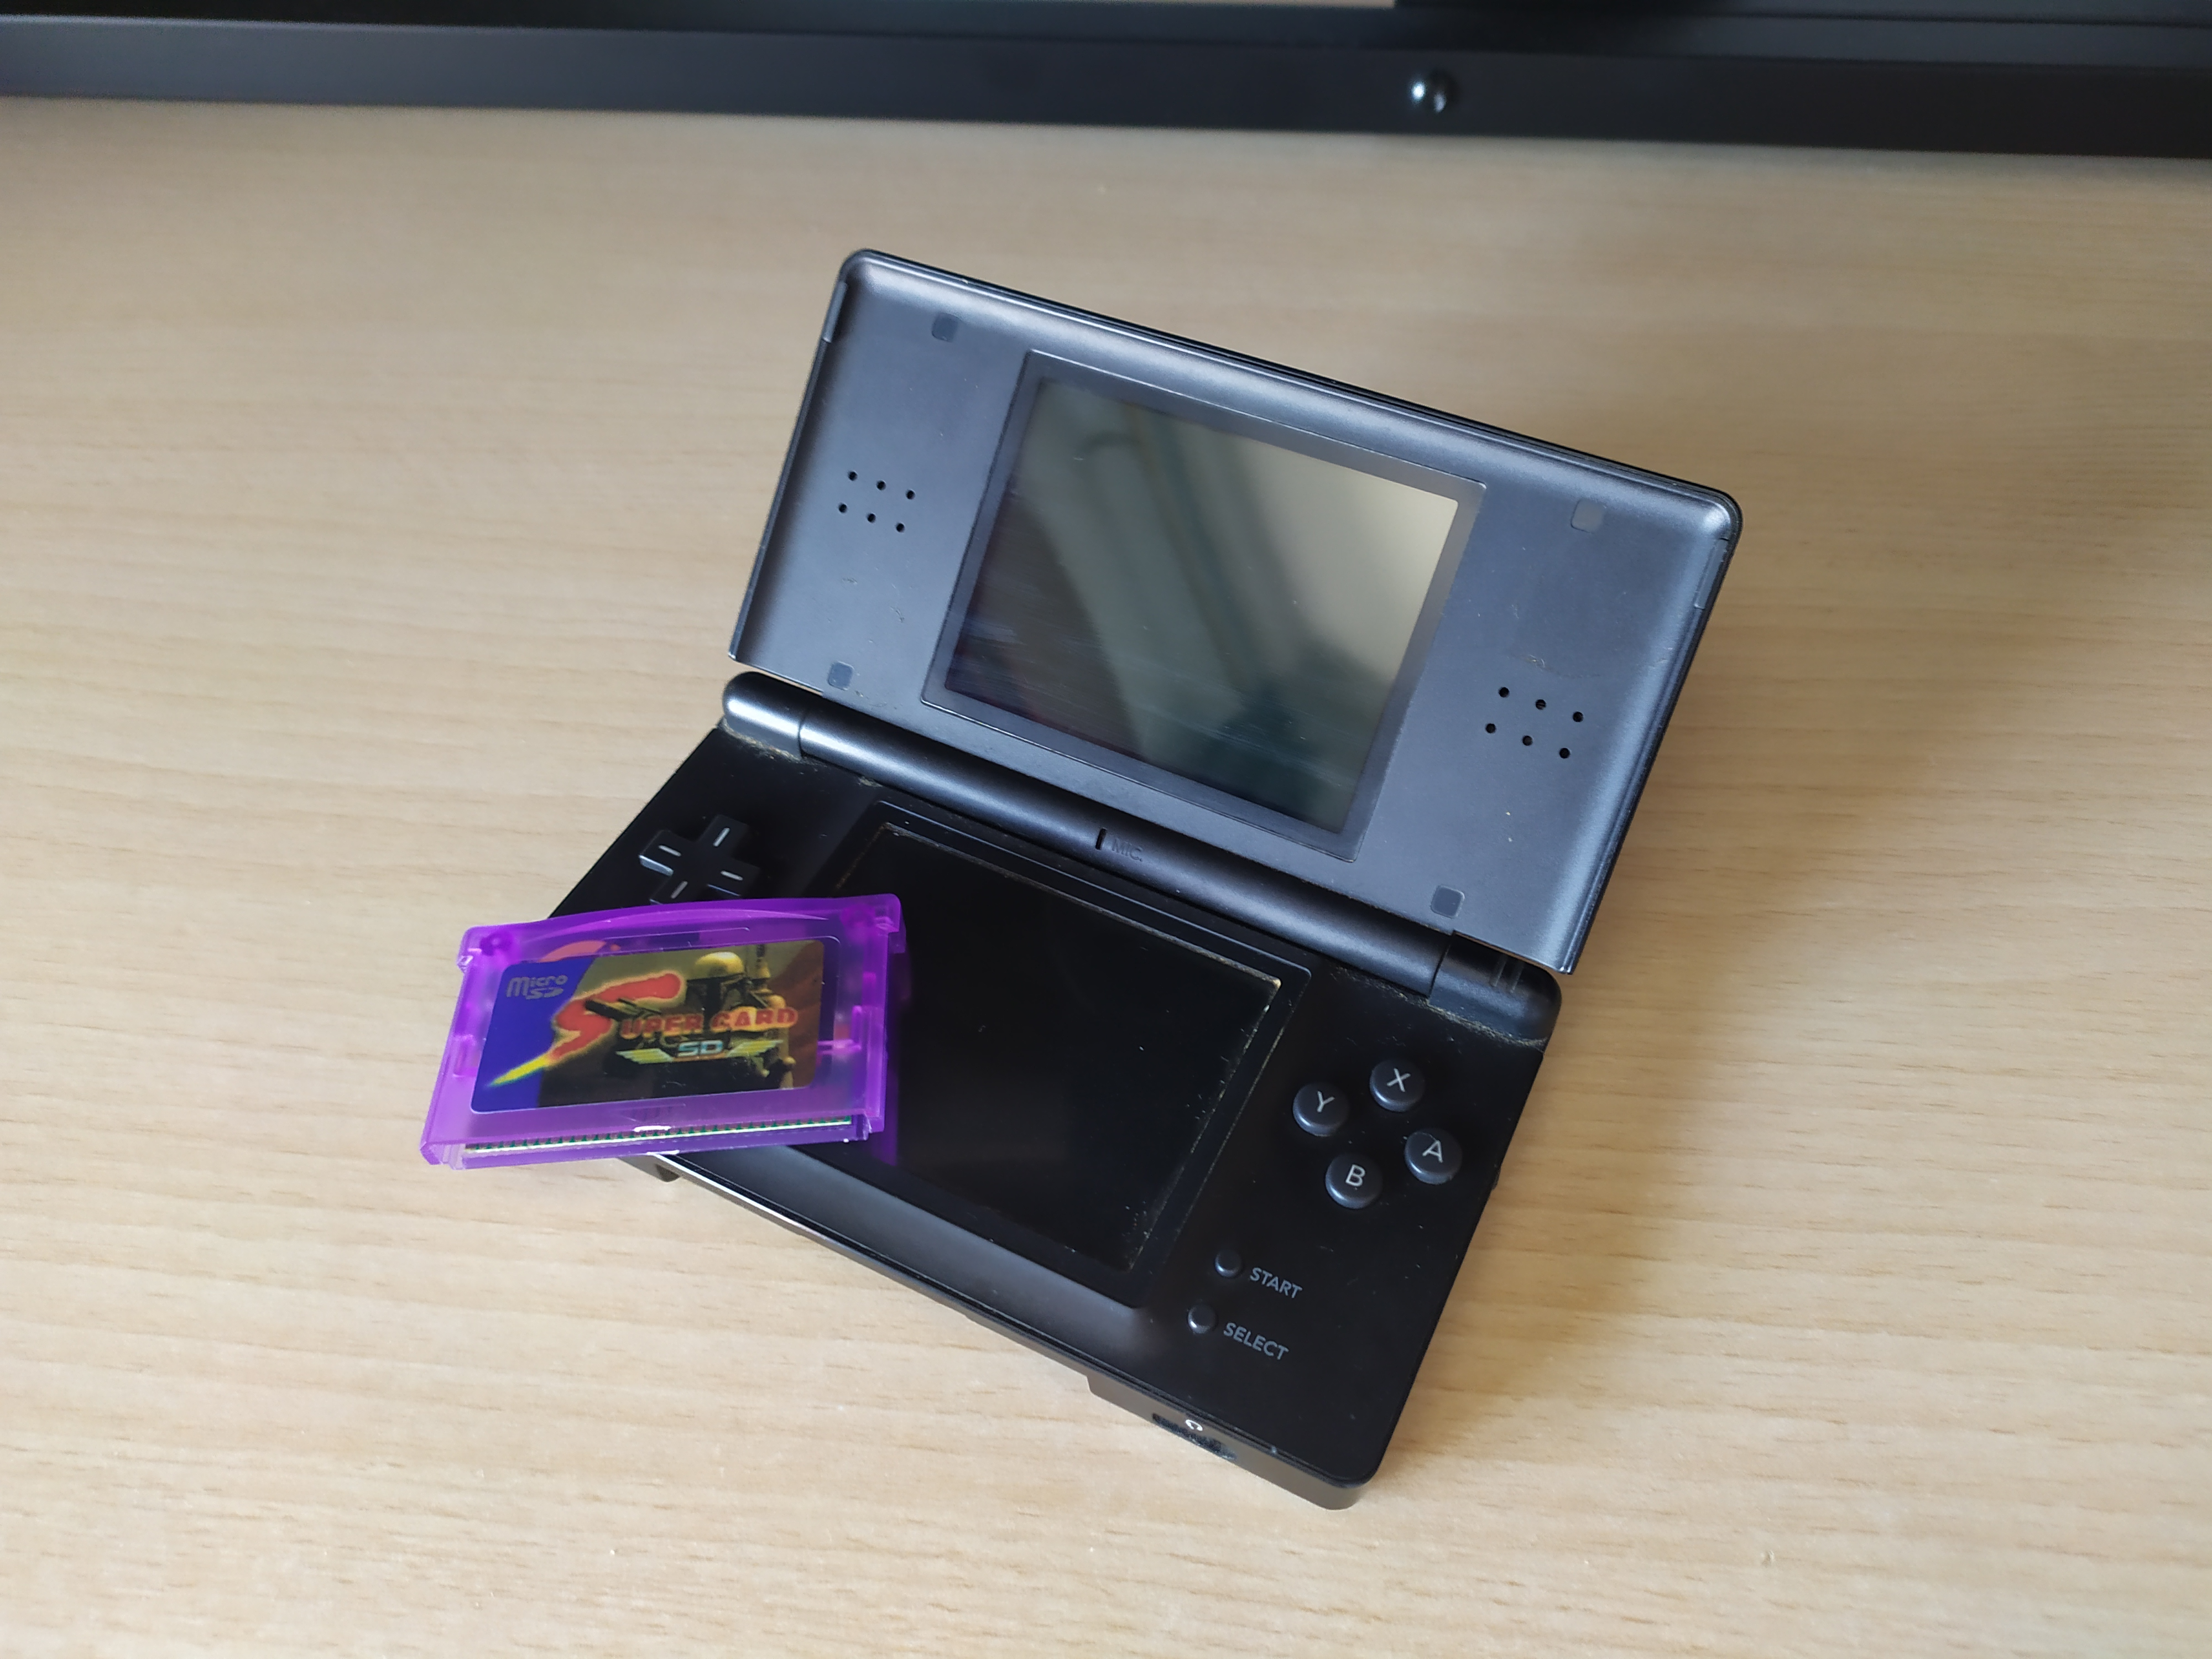
\includegraphics[height=7cm]{capitulos/capitulo1/nintendo_ds.jpg}
	\caption{Consola retrocompatible con la Game Boy Advance, la Nintendo DS Lite.}
	\label{fig:nintendo_ds}
\end{figure}

\vspace{1cm}

\begin{figure}[h]
	\centering
	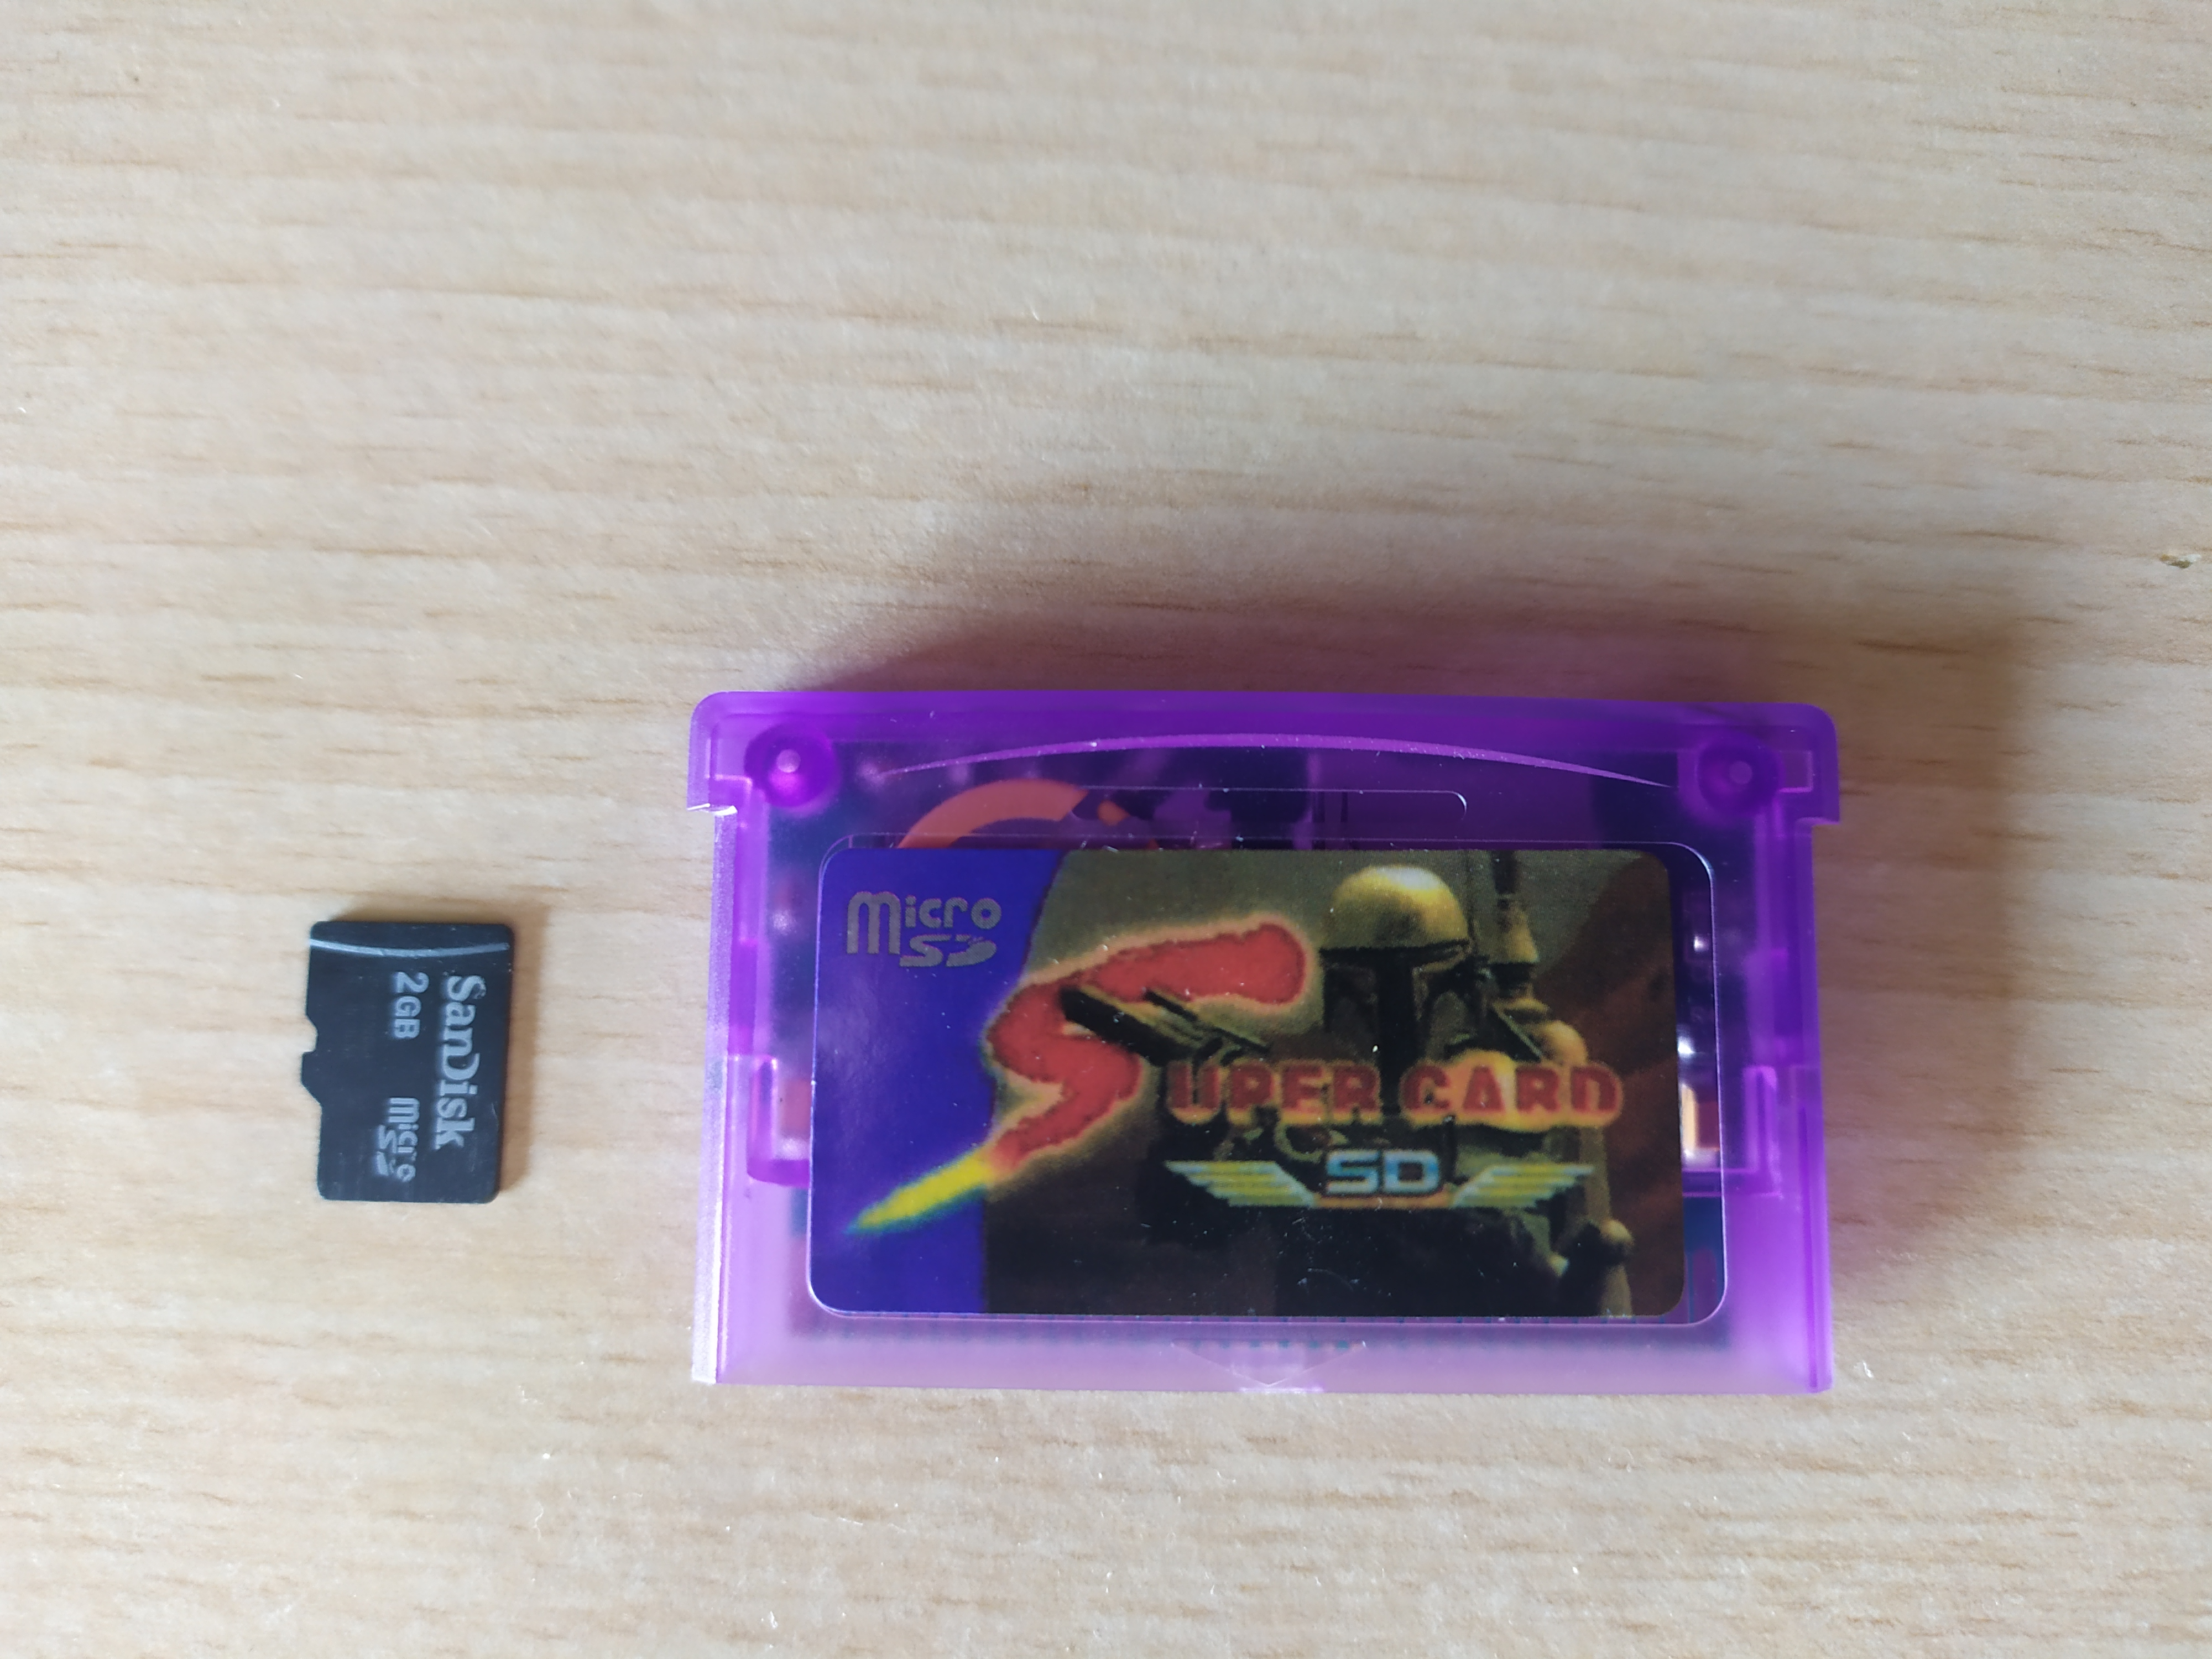
\includegraphics[height=6cm]{capitulos/capitulo1/supercard.jpg}
	\caption{Cartucho \textit{Supercard}.}
	\label{fig:supercard}
\end{figure}
\FloatBarrier

\section{Estructura del proyecto}
Este documento tiene como finalidad mostrar la solución desarrollada al problema propuesto, comentando a su vez las diversas características que tiene la Game Boy Advance. Dado que será necesario conocer varios conceptos antes de comentar el desarrollo del juego, la estructura del proyecto comenzará describiendo la arquitectura de la GBA y las opciones que ofrece.

En el Capítulo \ref{sec:arquitectura} se comentarán brevemente las características de los dos procesadores que utiliza la consola nipona y el papel que tiene cada uno en el dispositivo.

Seguidamente, se expondrán los registros principales y las funciones de cada uno. Entre ellas se encuentran, por ejemplo, la configuración de la pantalla y del sonido, las transferencias de acceso a directo a memoria y la comunicación con otros dispositivos.

Teniendo una idea de los registros que el desarrollador necesitará conocer para programar en el dispositivo, se explicarán los modos que ofrece la unidad de procesamiento de imágenes de la consola (\textit{PPU} ó \textit{Picture Processing Unit}). Se combinará la explicación de los diferentes modos con pequeñas demostraciones para facilitar la comprensión. Además, se introducirán al lector algunos conceptos matemáticos necesarios para comprender el funcionamiento de algunas de las funciones de la \textit{PPU}.

Partiendo de la base previa, en el Capítulo \ref{sec:desarrollo}, se detallarán los requisitos y especificaciones del proyecto, entre los que se incluirán varios diagramas. De forma adicional, se resaltarán algunos aspectos del desarrollo que distinguen a la Game Boy Advance con respecto a otros dispositivos.

En la fase final del informe, en concreto en el Capítulo \ref{sec:final}, se presentará la solución desarrollada para el proyecto, describiéndose el funcionamiento del juego. Se mostrará también cómo se ha probado el software en el hardware real, detallando el procedimiento a seguir.

Una vez descrito el estado actual del juego, en el Capítulo \ref{sec:conclusion} se expondrán las conclusiones detallando los conocimientos adquiridos y la experiencia de desarrollar un juego para la Game Boy Advance. Adicionalmente, se comentarán varias de las funcionalidades y mejoras descartadas para el proyecto en la fase de prototipado (de cada iteración) que podrán servir como líneas de trabajo en un futuro.

Finalmente, en los apéndices se incluirán información adicional de los registros y funciones del sistema, estructura del proyecto a nivel de código, varias imágenes mostrando el juego en funcionamiento y varios \textit{scripts} utilizados para facilitar el desarrollo del producto final.
